% !TeX program = xelatex
% !BIB program = bibtex
% !TeX encoding = UTF-8
\documentclass[preprint,12pt,nonatbib]{elsarticle}

\ifdefined\synctex
  \synctex=1
\fi

\usepackage{amssymb}
\usepackage{amsmath}
\usepackage[a4paper,margin=1in]{geometry}
\usepackage{graphicx}
\usepackage{booktabs}
\usepackage{subcaption}
\usepackage{caption}
\usepackage{float}
\usepackage{algorithm}
\usepackage{algpseudocode}
\usepackage{multirow}
\usepackage{array}
\usepackage{enumitem}
\usepackage{needspace}
\usepackage[natbibapa]{apacite}
\usepackage[hidelinks]{hyperref}
\hypersetup{pdfauthor={},pdfsubject={},pdfkeywords={}}
\usepackage{fontspec}
\emergencystretch=2em

\graphicspath{{./}}
\journal{Expert Systems with Applications}

\setcounter{topnumber}{3}
\setcounter{bottomnumber}{2}
\setcounter{totalnumber}{5}
\renewcommand{\topfraction}{0.9}
\renewcommand{\bottomfraction}{0.8}
\renewcommand{\textfraction}{0.07}
\renewcommand{\floatpagefraction}{0.8}

\renewcommand{\algorithmicrequire}{\textbf{Require:}}
\renewcommand{\algorithmicensure}{\textbf{Ensure:}}

\captionsetup[figure]{name=Fig.}
\captionsetup[table]{name=Tab.}

\newcommand{\figref}[1]{Fig.\nobreakspace\ref{#1}}
\newcommand{\tabref}[1]{Tab.\nobreakspace\ref{#1}}

\clubpenalty=10000
\widowpenalty=10000

\begin{document}

\begin{frontmatter}

\title{Reinforcement Learning-Based Computer Numerical Control Motion Planning with Adaptive Preview and Jerk-Constrained Action Projection}

\begin{abstract}
Two-step computer numerical control (CNC) motion planning fixes the geometry of computer-aided manufacturing (CAM) tool paths before feedrate scheduling, limiting adjustment within the tolerance band. We propose the Jerk-constrained Neural Numerical Controller (J-NNC), which jointly selects steering, feedrate and Adaptive Preview in a closed loop. The policy is learned through proximal policy optimization and fitting to recorded feasible actions. A kinematic constraint module (KCM) converts these decisions into planar motion satisfying kinematic constraints, allowing trajectory shape and feedrate to be adjusted together. On a 44.420514 m closed path, it completed ordered traversal, braking and rest in 444.177 s. Complete execution time was 1.008 s shorter than for a two-step planner. Speed deficit at every one of the 34 corners was no greater than for that planner or a trained two-action controller. On an 84-corner dense path, execution time was reduced by 25.65\% relative to two-step planning and 6.07\% relative to the fastest valid two-action result. The trajectories and motion profiles show turning before the corner, feedrate recovery and sustained near-limit cruising within the one-sided 1.25 mm Euclidean tolerance.
\end{abstract}

\begin{keyword}
computer numerical control \sep reinforcement learning \sep Adaptive Preview \sep jerk-constrained action projection
\end{keyword}

\end{frontmatter}

\section{Introduction}
\label{sec:introduction}
Computer numerical control (CNC) motion planning converts tool paths into executable commands subject to contour and kinematic limits. Conventional two-step planning smooths the geometry and then schedules feedrate along the resulting curve~\citep{Sun2022,Yan2023}. Fixing the geometry restricts how the scheduler can distribute corner transitions within the tolerance band~\citep{Erkorkmaz2001,Lee2011}. At consecutive corners, trajectory curvature and feedrate jointly determine acceleration and jerk.

\subsection{Related work}
Geometric smoothing provides explicit control over corner shape and contour error. \citet{Sencer2014} optimize quintic B\'ezier corner blends for low curvature and schedule S-curve feed transitions subject to drive acceleration and tangential jerk limits. Other smoothing methods address curvature continuity and axis jerk limits~\citep{Fan2015,Zhang2018}; short segments also require control of overlapping transitions~\citep{Hu2024,Yan2023}. Global fitting and filtering coordinate multiple blocks~\citep{Song2021,Yang2015}. Feedrate methods further address normal jerk, drive and chord-error constraints, using upcoming geometry to regulate motion~\citep{Zhang2021,Wu2022,Tsai2010,Song2020,Zhao2013}. These approaches use upcoming geometry while retaining a predefined geometric construction.

Integrated planning methods coordinate geometric smoothing with the motion constraints. Kinematic corner smoothing and integrated acceleration/deceleration interpolation directly coordinate corner motion~\citep{Tajima2016,Tsai2016}. Related formulations address minimum-time cornering, vibration suppression and driving-force limits~\citep{Duan2016,Sencer2015,LiDriving2017}. For mixed line--arc paths, \citet{Li2023} overlap adjacent segment motions and adjust kinematic parameters using a variable jerk-limited feed profile. Their formulation explicitly constrains resultant acceleration and jerk and controls corner error. Five-axis interpolation also addresses feedrate fluctuation and computational efficiency~\citep{Sun2024}. Here, a learned local rule jointly selects steering, feedrate and guide-target distance.

\citet{Li2020} introduced a Neural Numerical Controller (NNC) trained by deep deterministic policy gradient to generate position commands. Its two outputs are direction-angle and step-length rates, denoted $\theta'_t$ and $l'_t$ in their action definition and accumulated in the command update. The observation includes nine forward rays, whose distances to the tolerance boundaries are capped at $r_{\max}=3\varepsilon_{\mathrm{NNC}}$. Here $\varepsilon_{\mathrm{NNC}}$ denotes that paper's error-constraint parameter. NNC therefore already observes upcoming geometry. Its contour-error-based learning objective and reported per-axis kinematic settings differ from the explicit planar projection used here. J-NNC samples reference geometry at fixed distances and learns the guide-target distance as a separate action. The observation sampling distances remain fixed. The original NNC, our evaluated NNC adaptation and the fixed-preview two-action controller with KCM are distinct controllers in the comparison.

Existing learning-based methods also correct neural-network action requests before execution. OptLayer finds an action close to a network prediction using a differentiable quadratic program with state-dependent linear constraints~\citep{Pham2018}. The present kinematic constraint module (KCM) instead projects a next-velocity request onto intersecting planar disks defined by vector velocity, acceleration and jerk limits. An additional release check verifies that acceleration can then decrease within the limits. Contour tolerance and ordered coverage are checked separately; the kinematic projection alone does not establish geometric feasibility over the complete path.

\subsection{Research gap and contributions}
The remaining problem is to coordinate local trajectory shaping, feedrate and the guide-target distance while maintaining executable planar motion. We propose the Jerk-constrained Neural Numerical Controller (J-NNC), which jointly selects steering, feedrate and Adaptive Preview from current geometric and kinematic observations. Learning combines proximal policy optimization (PPO)~\citep{Schulman2017PPO} with fitting to recorded feasible actions. The KCM converts the combined request into interpolation commands. \figref{fig:comparison_arch} contrasts this framework with two-step planning.

\begin{figure}[htbp]
\centering
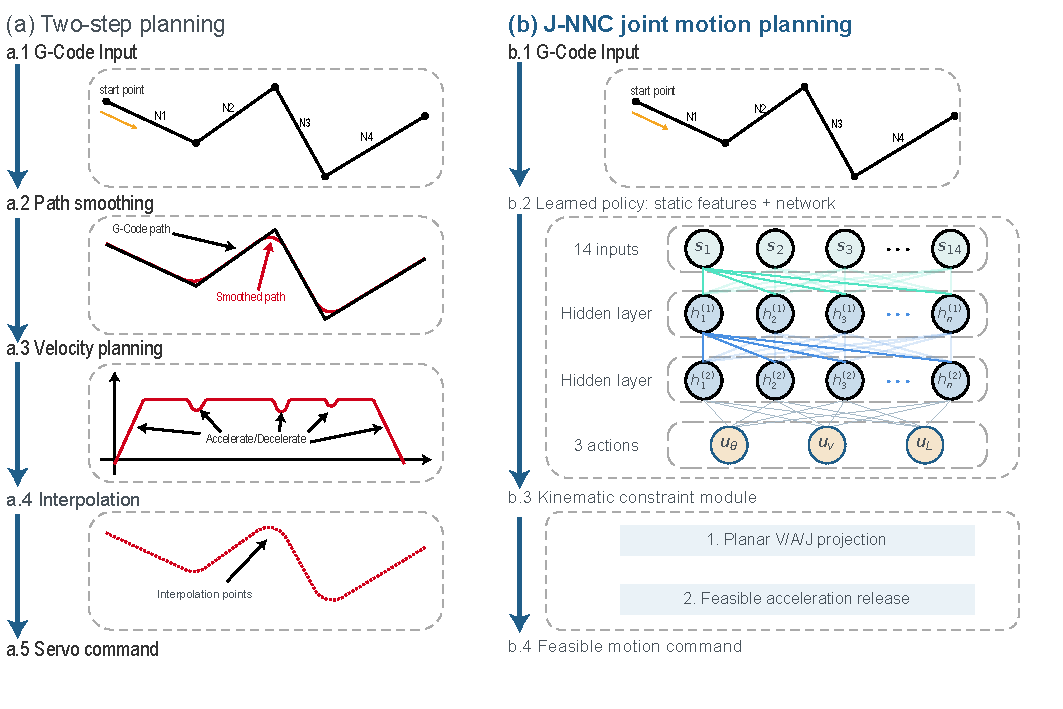
\includegraphics[width=0.9\linewidth]{Figure_1.pdf}
\caption{Conventional two-step planning and J-NNC joint motion planning. The policy uses 14 current inputs to select three actions. The KCM converts their combined request into feasible planar motion. In the diagram, $N_i$ labels a path block, $s_i$ is an input component, and $h_i^{(j)}$ is the output of unit $i$ in hidden layer $j$, with $n$ denoting the last unit. The outputs $u_\theta,u_v,u_L$ request steering, feedrate and preview, respectively. V/A/J denotes velocity, acceleration and jerk.}
\label{fig:comparison_arch}
\end{figure}

\begin{samepage}
The main contributions are as follows:
\begin{enumerate}
\item[(1)] A three-action formulation coordinates steering, feedrate and Adaptive Preview within the tolerance band, separating learned guide-target selection from fixed geometric observation sampling.
\item[(2)] A KCM combines projection onto planar velocity disks with checks on subsequent acceleration reduction to enforce velocity, acceleration and jerk limits on the executed commands.
\item[(3)] Complete executions on a long closed path and a corner-dense path compare traversal time and all-corner speed deficit under common contour and motion limits. The evaluation includes ordered coverage, braking and rest. The separate comparison with equal PPO budgets yielded time differences within the numerical sensitivity margin.
\end{enumerate}
\end{samepage}

Section 2 defines the planning problem and its constraints. Section 3 presents the method, and Section 4 reports the experimental settings, main results and comparison with fixed-preview control. Section 5 concludes the paper.

\section{Problem Formulation}
\label{sec:problem_formulation}
The planning problem is defined by the reference path, contour tolerance and constraints on the executed motion.

\subsection{Tool Path and Geometric Feasible Region}
Consider a discrete sequence of cutter-location points generated by a CAM system,
\begin{equation}
P_{\mathrm{raw}}=\{p_1,p_2,\dots,p_N\},
\end{equation}
Here $P_{\mathrm{raw}}$ is the reference path, $N$ is the number of cutter-location points, and $p_i\in\mathbb{R}^2$ is point $i$ in the two-dimensional interpolation plane. The prescribed line and arc segments connect these points. Its Cartesian axes are denoted by $X$ and $Y$. Let $\varepsilon$ denote the full width of the contour-tolerance band. Offsetting the reference path by $\varepsilon/2$ on each side defines the geometric feasible region $\Omega$ for a position $x$:
\begin{equation}
\Omega=\{x\mid d(x,P_{\mathrm{raw}})\leq \varepsilon/2\},
\label{eq:feasible_region}
\end{equation}
where $d(x,P_{\mathrm{raw}})$ is the minimum Euclidean distance from $x$ to the finite reference path, including its line and arc segments. The one-sided tolerance is therefore $\varepsilon/2$. Within this band, the controller can adjust the local trajectory to smooth corner transitions while maintaining contour accuracy.

\begin{figure}[htbp]
\centering
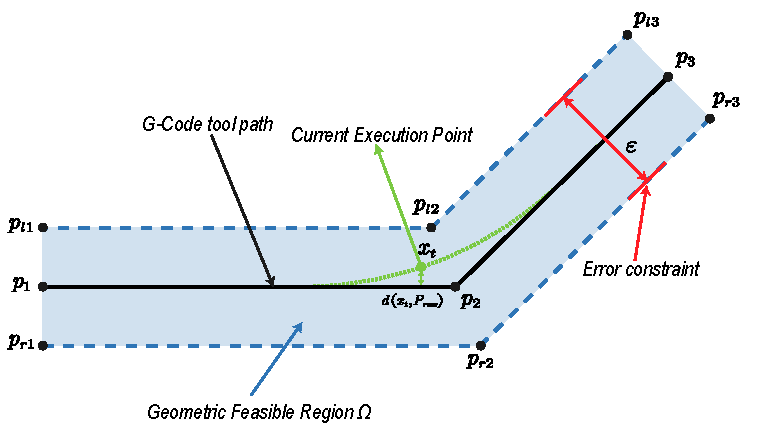
\includegraphics[width=0.9\linewidth]{Figure_2.pdf}
\caption{Geometric feasible region formed by the reference path and the contour tolerance band. Points $p_{li}$ and $p_{ri}$ mark the left and right boundaries associated with reference point $p_i$; $x_t$ is the current execution point at decision index $t$.}
\label{fig:feasible_region}
\end{figure}

The reference path is parameterized by arc length for closed-loop control. Tracking variables and forward geometry are extracted at the current projected arc length $\ell_t$ at decision index $t$ to form the observation. An ordered sequence of gates preserves traversal order where different portions of the closed path lie close together.

\subsection{Constrained Action Decision Formulation}
At each decision interval $\Delta t$, the policy receives the current state $s_t$ and returns an action $u_t$. The execution layer converts this request into feasible planar motion at interval $h$. During training, the environment updates the position and motion variables and returns reward $r_t$. For policy $\pi$, discount factor $\gamma\in[0,1]$ and final decision index $H$, the constrained decision problem is
\begin{equation}
\max_{\pi}\ \mathbb{E}_{\pi}\!\left[\sum_{t=0}^{H}\gamma^t r_t\right],
\end{equation}
where $\mathbb{E}_{\pi}$ denotes expectation over trajectories generated by $\pi$. At execution index $k$, the position is $x_k$ and the planar velocity, acceleration and jerk vectors are $v_k,a_k,j_k$. Their magnitude limits are $V_{\max},A_{\max},J_{\max}$, respectively, and $\|\cdot\|_2$ denotes the Euclidean norm. The constraints are $x_k\in\Omega$ and
\begin{equation}
\|v_k\|_2\leq V_{\max},\qquad \|a_k\|_2\leq A_{\max},\qquad \|j_k\|_2\leq J_{\max}.
\end{equation}
These bounds apply to planar vectors and include the acceleration and jerk associated with turning. The motion variables are reconstructed from executed positions as
\begin{equation}
v_k=\frac{x_k-x_{k-1}}{h},\quad a_k=\frac{v_k-v_{k-1}}{h},\quad j_k=\frac{a_k-a_{k-1}}{h}.
\label{eq:physical_differences}
\end{equation}
The initial velocity and acceleration are zero. Derivatives of scalar speed omit changes in direction and cannot fully assess these vector constraints. Heading and curvature describe the resulting trajectory; no separate angular-axis limits are imposed.

A successful execution traverses the entire reference path in order and keeps every command interval within the Euclidean tolerance band. It also completes braking and remains at rest for at least 20 ms. Complete execution time includes startup, traversal, braking and this rest period, so the comparison covers the same complete task.
\section{Methodology}
\label{sec:methodology}
\subsection{Overall Framework}
Adaptive Preview is the preview distance selected by the policy from the current state.

Motion planning for mixed tool paths is formulated as a closed-loop reinforcement learning problem. The policy acts in a path-simulation environment with prescribed contour and kinematic limits. At each decision cycle, the environment constructs the state from tracking error, motion variables and forward geometry. The policy supplies steering, feedrate and Adaptive Preview requests, which the KCM converts into executable planar motion. The executed motion updates the state and provides reward feedback during training.

\figref{fig:framework} shows the control loop. Preview selects the forward guide target, steering corrects its direction, and feedrate sets the requested speed. The execution layer constrains the next velocity using the current velocity and acceleration vectors. Evaluation uses the same feedback loop with fixed policy parameters. In the diagram, $f_\theta$ maps the current state $s$ to action $u$, and $\theta$ denotes its fitted parameters. The decoded requests $\alpha,F,L$ are steering correction, feedrate and preview distance. Subscripts are omitted for the held state and action; $v_{k+1}$ is the next executed velocity.

\begin{figure}[htbp]
\centering
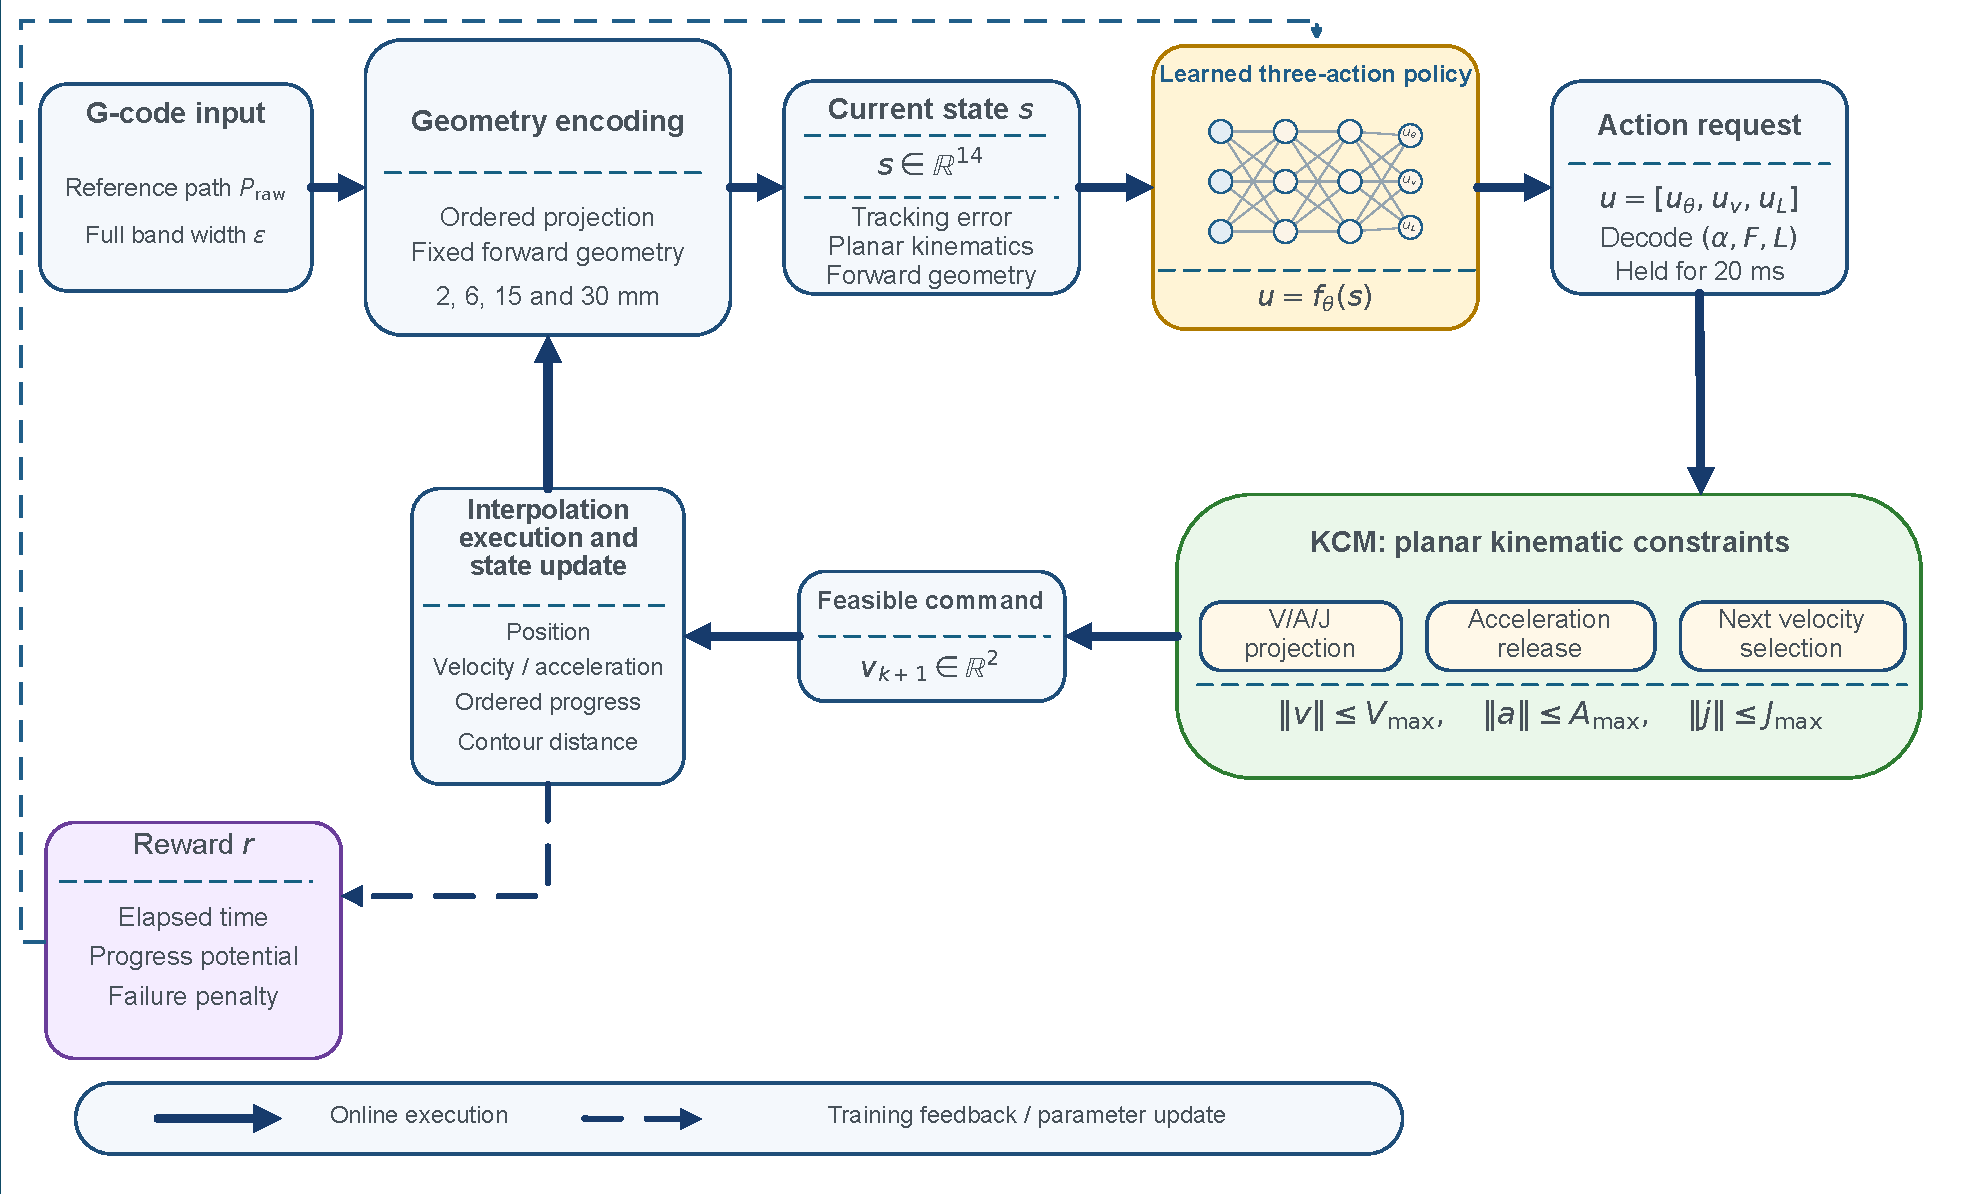
\includegraphics[width=0.9\linewidth]{Figure_3.pdf}
\caption{J-NNC control loop. Forward geometry sampled at fixed distances and current motion variables form the 14-dimensional state. The policy outputs steering, feedrate and Adaptive Preview requests, and the KCM determines feasible planar commands. The dashed outer connection represents training feedback and parameter updates.}
\label{fig:framework}
\end{figure}

\subsection{State Design}
The controller uses a 14-dimensional observation of the current state. Tracking and motion variables describe the present motion, while near and far reference points describe upcoming geometry. The columns of $R_h$ are the current heading unit vector and its left normal. Let $t_r,n_r$ denote the local reference unit tangent and unit normal, and let $p(\ell)$ denote a reference point. The current position, velocity and acceleration vectors are $x,v,a$, with time indices omitted. Here $\ell$ is the projected arc length, $d$ is a forward sampling distance, and $\theta_r,\theta_h$ are the reference-tangent and current-heading angles. The input is
\begin{equation}
\begin{split}
s={}&[e_n/1.25,\ R_h^{\mathsf T}v/100,\ R_h^{\mathsf T}a/2000,\ q_{30}^{\parallel},\ \sin(\theta_r-\theta_h),\\
&\{R_h^{\mathsf T}[p(\ell+d)-x]/15\}_{d\in\{2,6,15\}},\ q_{30}^{\perp}],
\end{split}
\label{eq:state14}
\end{equation}
where $e_n=[x-p(\ell)]\cdot n_r$ is the signed normal tracking error. The dimensionless far-reference components $q_{30}^{\parallel}$ and $q_{30}^{\perp}$ are the tangential and normal projections of the displacement to the point 30 mm ahead:
\begin{equation}
q_{30}^{\parallel}=\frac{[p(\ell+30)-p(\ell)]\cdot t_r}{30},\qquad
q_{30}^{\perp}=\frac{[p(\ell+30)-p(\ell)]\cdot n_r}{30}.
\end{equation}
Lengths are expressed in millimeters. The two far-reference components are expressed in the reference frame. Velocity, acceleration and the three near-reference point pairs are expressed in the heading frame. The 14 inputs comprise one tracking error, four kinematic components, one heading sine, six near-point coordinates and two far-reference components.

The near-reference points describe the local transition and recovery, while the 30 mm displacement provides information about geometry farther ahead. These fixed sampling distances are distinct from the preview distance selected by the action. Blending adjacent estimates of reference progress reduces observation jumps at segment boundaries without changing the ordered coverage sequence. The observation excludes elapsed time, global coordinates, corner identifiers, remaining path length and previous actions. The policy stores neither a recurrent state nor an observation history. The static nonlinear features in \ref{app:learning} depend only on these 14 current inputs.

\subsection{Action Space and Kinematic Constraint Module}
At decision $t$, the action $u_t$ contains the normalized steering, feedrate and preview components $u_{\theta,t},u_{v,t},u_{L,t}$, each clipped to $[-1,1]$:
\begin{equation}
u_t=[u_{\theta,t},u_{v,t},u_{L,t}].
\end{equation}
The normalized outputs are mapped to physical requests as
\begin{equation}
\alpha_t=\frac{\pi}{2}u_{\theta,t},\qquad
F_t=50(1+u_{v,t}),\qquad
L_t=6.4+5.6u_{L,t}.
\label{eq:decode}
\end{equation}
Here $\alpha_t$ is a steering correction in radians, $F_t$ is the requested feedrate in mm/s, and $L_t\in[0.8,12]$ mm is the Adaptive Preview distance. The steering action corrects direction rather than commanding angular velocity. The three requests are held for 20 ms, while the guide direction and motion are updated at the smaller integration interval $h$.

The guide direction points from the current position toward the reference point selected by preview distance $L$. Steering corrects this direction, and filtering smooths its changes between interpolation steps. The filtered direction and feedrate $F$ define the desired velocity. Using velocity and acceleration feedback, the execution layer forms a next-velocity request for KCM projection. A release check verifies that acceleration can subsequently decrease within the constraints (\ref{app:kcm}). Contour tolerance and complete ordered coverage are checked separately.

\subsection{Reward Design}
The learning objective combines elapsed execution time, progress shaping and a failure penalty:
\begin{equation}
r_t=-\Delta t_t+\Phi_{t+1}-\Phi_t-\mathbf{1}_{\mathrm{failure}}P_t,
\qquad \Phi_t=\frac{\ell_t-\ell_{\mathrm{total}}}{V_\Phi}.
\label{eq:reward_total}
\end{equation}
Here $\Delta t_t$ is the actual duration of decision step $t$, $\Phi_t$ is a progress potential, $\ell_{\mathrm{total}}$ is total reference length, and $V_\Phi$ scales distance to time. The indicator $\mathbf{1}_{\mathrm{failure}}$ is one on failure and zero otherwise; $P_t$ is the failure penalty. The last PPO training stage uses $V_\Phi=100$ mm/s and zero terminal potential. Failure incurs $P_t=5+\ell_{\mathrm{rem}}/100$ seconds, where $\ell_{\mathrm{rem}}$ is the remaining reference distance in millimeters. For successful undiscounted episodes with the same initial state, the potential differences sum to a constant. Maximizing the return therefore minimizes complete execution time. The learning procedure is described in \ref{app:learning}. Performance is evaluated using executed motion and completion time rather than reward values.

Policy learning combines PPO~\citep{Schulman2017PPO} with fitting to recorded feasible actions. The fixed policy combines a neural network with static features of the same 14 inputs; its complete expression and learning settings appear in \ref{app:learning}.

\section{Experiments and Results}
\label{sec:experiments}
\subsection{Experimental Settings}
The experiments assess motion feasibility and the effect of joint trajectory shaping and feedrate regulation on complete execution time. The long closed path has a reference length of 44.420514 m, and all 34 corners are included in the analysis. Figure~\ref{fig:case_execution} identifies its longest and shortest continuous straight sections (2262.742 and 80 mm) and extreme included angles ($45.000^\circ$ and $175.679^\circ$). It also marks two $90^\circ$ arcs with radii of 600 and 800 mm. Continuous straight lengths are measured after merging adjacent collinear blocks with the same direction, including blocks spanning the closed-path junction. The enlarged view of the shortest straight section uses a 10 mm Cartesian grid. A second closed path is 1438.009 mm long and contains 84 corners (\figref{fig:ablation_dense}a).

The paths combine long and short straight sections, different corner angles and line--arc transitions. Long straight sections assess sustained cruising, varied angles assess turning and feedrate recovery, and dense successive corners assess interaction between transitions. Complete execution time measures efficiency; contour deviation and vector velocity, acceleration and jerk utilization assess constraint compliance; corner speed deficit measures local deceleration.

The primary results use a 1 ms interpolation interval. The full tolerance-band width is $\varepsilon=2.5$ mm, corresponding to a one-sided Euclidean tolerance of 1.25 mm. All methods use the same planar vector limits: $V_{\max}=100$ mm/s, $A_{\max}=2000$ mm/s$^2$ and $J_{\max}=62500$ mm/s$^3$. The learned constrained controllers update their action requests every 20 ms. Successful execution requires complete ordered traversal, geometric feasibility throughout each command interval, full braking and at least 20 ms of rest. The long-path evaluation includes all 2362 ordered gates and the final segment. A supplementary evaluation at 0.5 ms checks that the time gains exceed the effects of execution resolution (\ref{app:resolution}).

The Neural Numerical Controller (NNC) comparison adapts the original direct-action checkpoint based on learned CNC smoothing~\citep{Li2020}. The evaluated controller uses 14 inputs and 1 ms decisions, removes angular-motion feedrate caps and uses no KCM. Position commands are recorded from rest for up to 1 s or until termination. Figure~\ref{fig:nnc_failure} evaluates this adaptation under the present constraints. The two-step planner schedules jerk-limited motion after quintic B\'ezier smoothing adapted from \citet{Sencer2014}; circular arcs retain their analytical form. No method receives a global feedrate reduction.

The two-action comparison retains steering and feedrate, with the same 14 inputs, execution layer and number of joint-action features (\ref{app:learning}). It receives separate fitting, parameter selection and PPO training. The selected controller completes both cases. Dense-case comparisons also retain the fastest valid two-action result, including models that fail on the long path.

For long-route corner $c$, let $\ell_c$ be its reference arc length and $\ell_k$ the ordered reference progress at execution step $k$. Integrated speed deficit $D_c$ is
\begin{equation}
D_c=h\sum_{k:\,|\ell_k-\ell_c|\leq10\ \mathrm{mm}}\max(100-\|v_k\|_2,0).
\label{eq:corner_deficit}
\end{equation}
This metric, measured in millimeters, captures both the magnitude and duration of speed reduction. All 34 complete corner windows are included, with numerical ties allowed within $10^{-7}$ mm. Near-limit cruising is defined throughout as $\|v_k\|_2\geq99$ mm/s. The utilization curves are $\|v\|_2/V_{\max}$, $\|a\|_2/A_{\max}$ and $\|j\|_2/J_{\max}$, reconstructed from executed planar positions using Eq.~\eqref{eq:physical_differences}. A value of one indicates the corresponding limit; the vector norms include the motion associated with changes in direction.

\begin{figure}[!htbp]
\centering
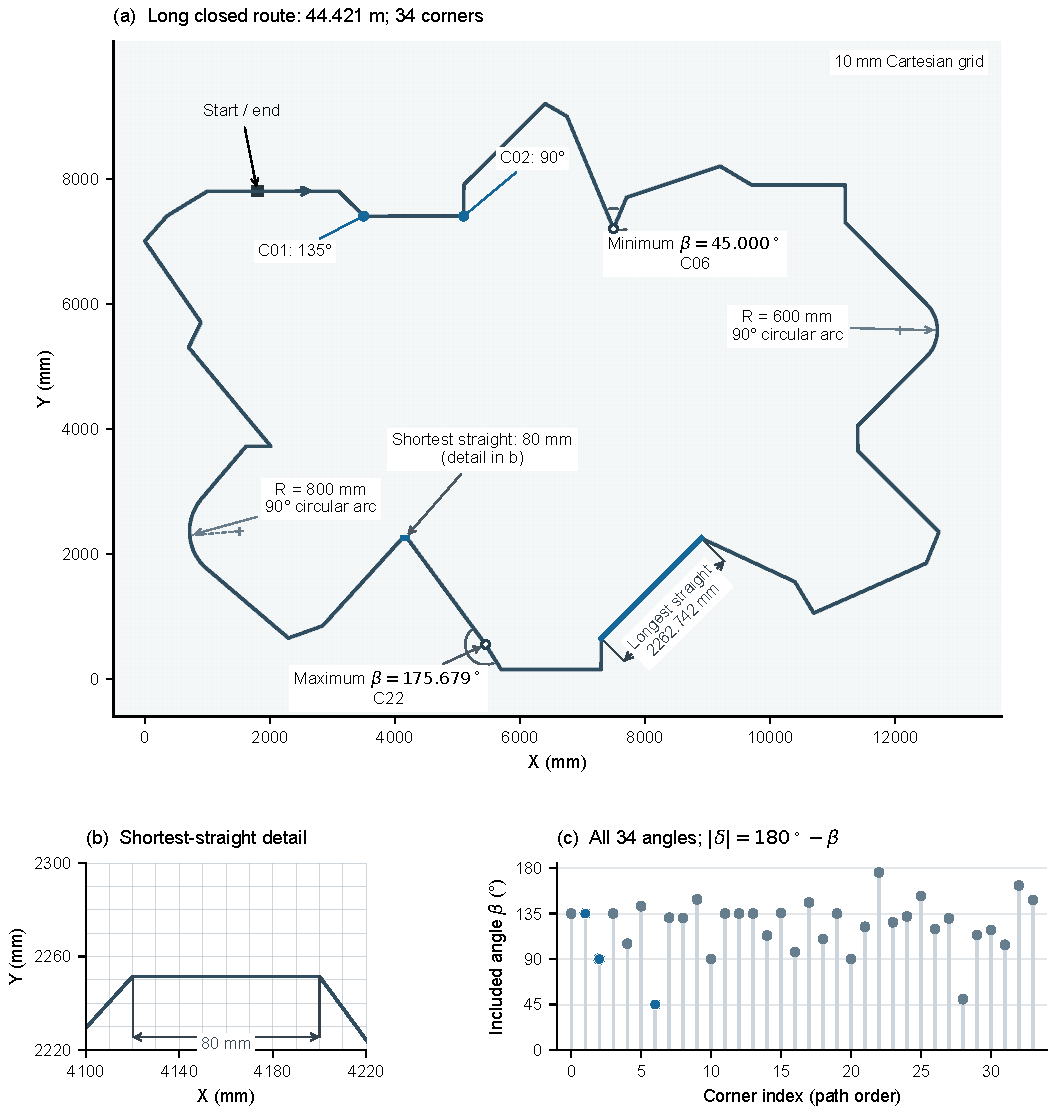
\includegraphics[width=0.98\linewidth,height=0.77\textheight,keepaspectratio]{Figure_4.pdf}
\caption{Long-path geometry and corner angles: (a) complete path with the longest and shortest continuous straight sections, extreme included angles and circular arcs; (b) enlarged shortest straight section on a 10 mm grid; (c) all 34 included angles. Here $\beta$ is the included corner angle, $\delta$ is the signed direction change, and $R$ is arc radius. C00--C33 identify corners in path order; C01, C02 and C06 are used in the local comparisons.}
\label{fig:case_execution}
\end{figure}

\subsection{Main Comparative Results}
J-NNC completed both paths within the common contour and planar kinematic limits (\tabref{tab:main_results}). Its complete execution time on the long path was 444.177 s, saving 1.008 s over two-step planning and 0.537 s over the selected two-action controller. On the dense path, J-NNC took 14.839 s, compared with 19.957 s for two-step planning, a reduction of 25.65\%. These times include startup, every corner transition, braking and terminal rest.

\begin{table}[htbp]
\centering
\caption{Feasibility and complete execution time at a 1 ms interpolation interval. Successful runs satisfy ordered traversal, contour tolerance throughout each command interval, planar V/A/J limits and terminal rest.}
\label{tab:main_results}
\small
\setlength{\tabcolsep}{3.5pt}
\begin{tabular}{lllrr}
\toprule
Case & Method & Feasible & Complete time (s) & \shortstack{Maximum contour\\deviation (mm)}\\
\midrule
Long path & \textbf{J-NNC} & Yes & \textbf{444.177} & 1.221862\\
 & Two-action & Yes & 444.714 & 1.095198\\
 & Two-step planner & Yes & 445.185 & 1.243758\\
 & NNC & No & --- & ---\\
\midrule
Dense case & \textbf{J-NNC} & Yes & \textbf{14.839} & 1.154901\\
 & Two-action & Yes & 15.875 & 1.121741\\
 & Two-step planner & Yes & 19.957 & 1.149675\\
 & NNC & No & --- & ---\\
\bottomrule
\end{tabular}
\par\smallskip
\begin{minipage}{0.98\linewidth}\footnotesize
Maximum contour deviation is evaluated throughout each command interval. NNC violates the acceleration and jerk limits; dashes indicate that no feasible complete result is available.
\end{minipage}
\end{table}

Figure~\ref{fig:nnc_failure} shows repeated constraint violations by the adapted NNC during the first 80 ms, including after startup. In the retained first-second records, peak acceleration was 20.70/29.54 times the limit on the long/dense paths; peak jerk was 841.69/1150.81 times the limit. J-NNC remained within the bounds. This adaptation therefore has no feasible complete execution time under the prescribed limits.

\begin{figure}[!htbp]
\centering
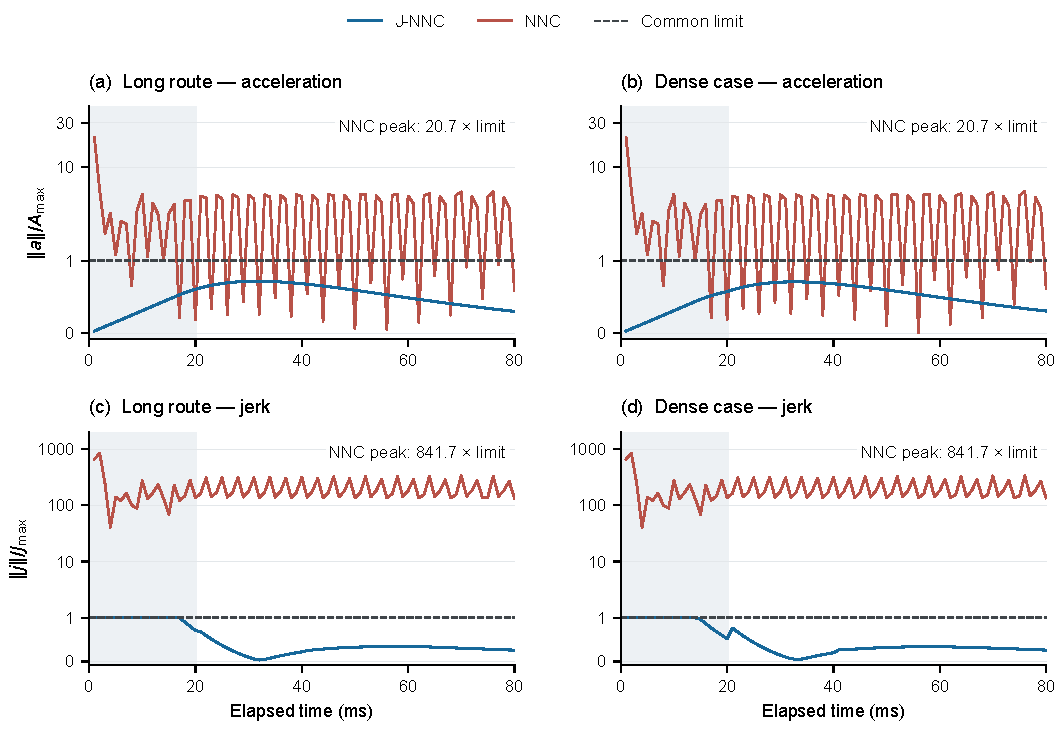
\includegraphics[width=0.98\linewidth]{Figure_5.pdf}
\caption{Constraint violations of the adapted NNC at 1 ms: normalized vector acceleration (a,b) and jerk (c,d) during the first 80 ms of each case. Shading marks the initial 20 ms, and dashed lines indicate the common limits. The vertical axes are linear from zero to one and logarithmic above one. Peak annotations apply only to the displayed interval. Curves are reconstructed from recorded planar positions.}
\label{fig:nnc_failure}
\end{figure}

Figure~\ref{fig:full_utilization} compares the methods at the selected $90^\circ$ corner C02 using common axes. J-NNC maintained a higher cornering speed within the same acceleration and jerk limits. Integrated speed deficit, which includes the magnitude and duration of deceleration, was 86.1\% lower than for two-step planning and 36.7\% lower than for two-action control. Complete V/A/J profiles, including terminal braking and rest, are provided in \figref{fig:complete_support}.

\begin{table}[htbp]
\centering
\caption{Kinematic-limit utilization over complete executions at 1 ms. Values are expressed as percentages of the common planar vector limits.}
\label{tab:utilization}
\small
\setlength{\tabcolsep}{3.5pt}
\begin{tabular}{llrrr}
\toprule
Case & Method & \shortstack{Mean $V$\\utilization} & \shortstack{95th-percentile $A$\\utilization} & \shortstack{95th-percentile $J$\\utilization}\\
\midrule
Long path & \textbf{J-NNC} & \textbf{99.939} & 0.678 & 0.370\\
 & Two-action & 99.870 & 0.731 & 0.536\\
 & Two-step planner & 99.716 & 0.625 & 0.004\\
\midrule
Dense case & \textbf{J-NNC} & \textbf{91.071} & 99.900 & 99.900\\
 & Two-action & 86.528 & 99.900 & 99.900\\
 & Two-step planner & 67.139 & 67.696 & 98.084\\
\bottomrule
\end{tabular}
\par\smallskip
\begin{minipage}{0.98\linewidth}\footnotesize
Statistics include all equally spaced samples during startup, traversal, braking and rest. The 95th percentiles describe the distribution over the full execution and do not represent peak utilization.
\end{minipage}
\end{table}

Table~\ref{tab:utilization} summarizes utilization over the complete executions. On the dense path, mean feedrate utilization was 67.139\% for two-step planning, 86.528\% for two-action control and 91.071\% for J-NNC. Both learned controllers had 95th-percentile acceleration and jerk utilization of 99.900\%. J-NNC achieved a higher mean feedrate under the same limits. The low acceleration and jerk percentiles on the long path reflect the large proportion of cruising. Figure~\ref{fig:full_utilization} shows utilization during the local corner transition.

\begin{figure}[!htbp]
\centering
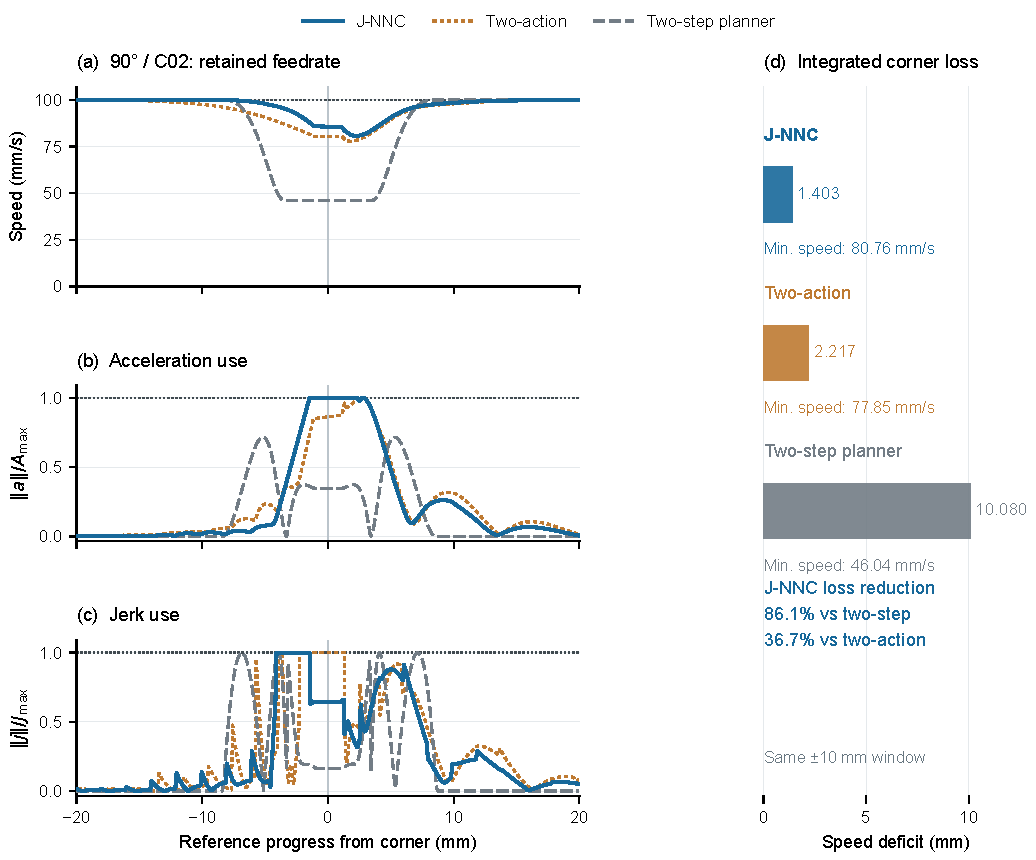
\includegraphics[width=0.98\linewidth,height=0.75\textheight,keepaspectratio]{Figure_6.pdf}
\caption{Motion at the selected $90^\circ$/C02 corner from the same 1 ms records. Panels (a)--(c) align speed, normalized vector acceleration and normalized vector jerk by reference progress; dotted horizontal lines indicate the common limits. Panel (d) gives integrated speed deficit and minimum speed within the common $\pm10$ mm window. The profiles span $\pm20$ mm to include approach and recovery.}
\label{fig:full_utilization}
\end{figure}

Figure~\ref{fig:local_shapes} compares the executed trajectories at the selected $135^\circ$, $90^\circ$ and $45^\circ$ corners. The upper row uses local coordinates $x$ along the incoming tangent and $y$ along the inward normal. These plotting coordinates are distinct from the position vector $x$ in the motion equations. The lower row enlarges the marked transition regions. Equal aspect ratios and common scales within each row allow direct comparison of the trajectory shapes. J-NNC began turning inward before the vertex and spread the direction change through the tolerance band, consistent with its higher cornering feedrate in \figref{fig:full_utilization}.

\begin{figure}[!htbp]
\centering
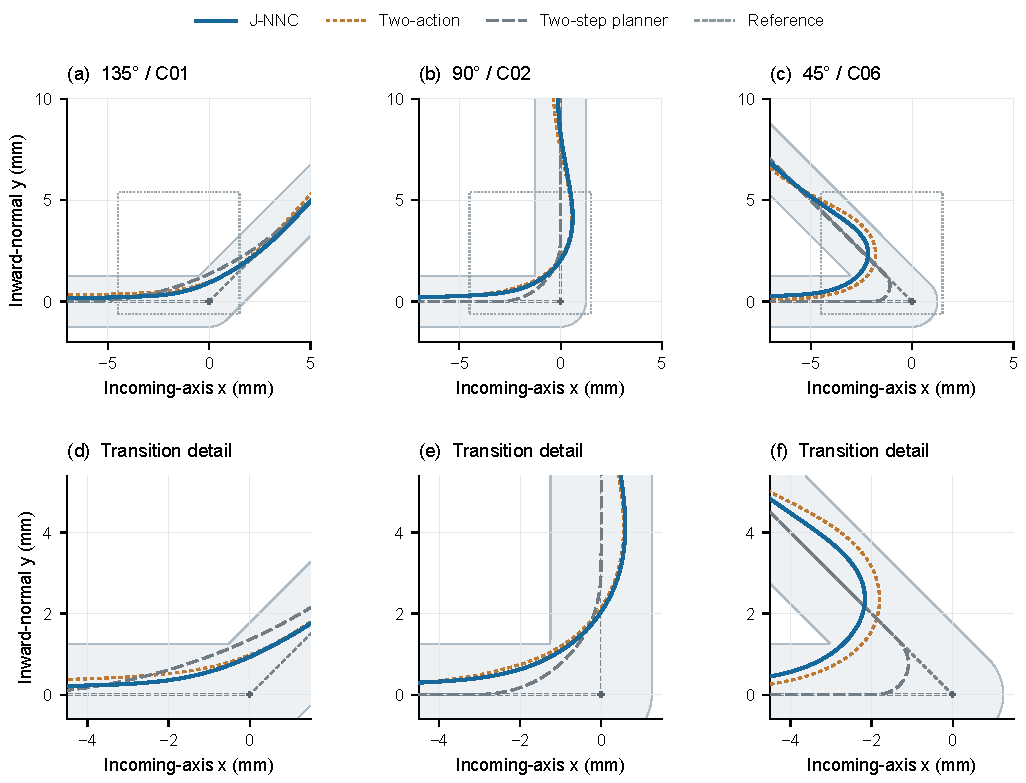
\includegraphics[width=0.98\linewidth,height=0.77\textheight,keepaspectratio]{Figure_7.pdf}
\caption{Executed trajectories at the selected $135^\circ$/C01, $90^\circ$/C02 and $45^\circ$/C06 corners. Panels (a)--(c) show approach and recovery; dotted rectangles mark the enlarged regions in (d)--(f). Shading indicates the 1.25 mm Euclidean tolerance band. Each row uses equal aspect ratios and common scales. The trajectories are extracted from the 1 ms executions of the corresponding controllers reported in Table~\ref{tab:main_results}.}
\label{fig:local_shapes}
\end{figure}

J-NNC traversed the $135^\circ$ corner at 100 mm/s. At the $90^\circ$ corner C02, its minimum speed was 80.76 mm/s, compared with 46.04 mm/s for two-step planning and 77.85 mm/s for two-action control. Integrated speed deficit was 10.080 mm for the two-step planner, 2.217 mm for the two-action controller and 1.403 mm for J-NNC. At the sharper C06 corner, the corresponding deficits were 13.321, 5.963 and 4.253 mm. J-NNC began turning inward before the vertex at all 34 long-path corners and all 84 dense-path corners.

The trajectory shapes and utilization profiles illustrate the coupling between geometry and feedrate. For a smooth trajectory, the signed normal acceleration $a_n$ satisfies $a_n=\|v\|_2^2\kappa$, where $\kappa$ is signed trajectory curvature; jerk during turning also depends on curvature variation along the trajectory. Steering and preview distribute the direction change, and feedrate adjusts the acceleration and jerk required to follow it. The displayed trajectories use limited outward recovery within the tolerance band and achieve lower speed deficit. Such outward displacement can provide additional turning space within the band; it is not directly rewarded.

Figure~\ref{fig:all_corners} reports the results for every corner on the long path. J-NNC had no greater integrated speed deficit than the two-step planner or trained two-action controller at any of the 34 corners, allowing numerical ties. Summed corner deficit decreased from 114.203 mm for two-step planning and 42.107 mm for two-action control to 13.902 mm for J-NNC. The cumulative full-path curves remain flat during near-limit cruising and show where additional deceleration occurs in the second half of the lap.

\begin{figure}[!htbp]
\centering
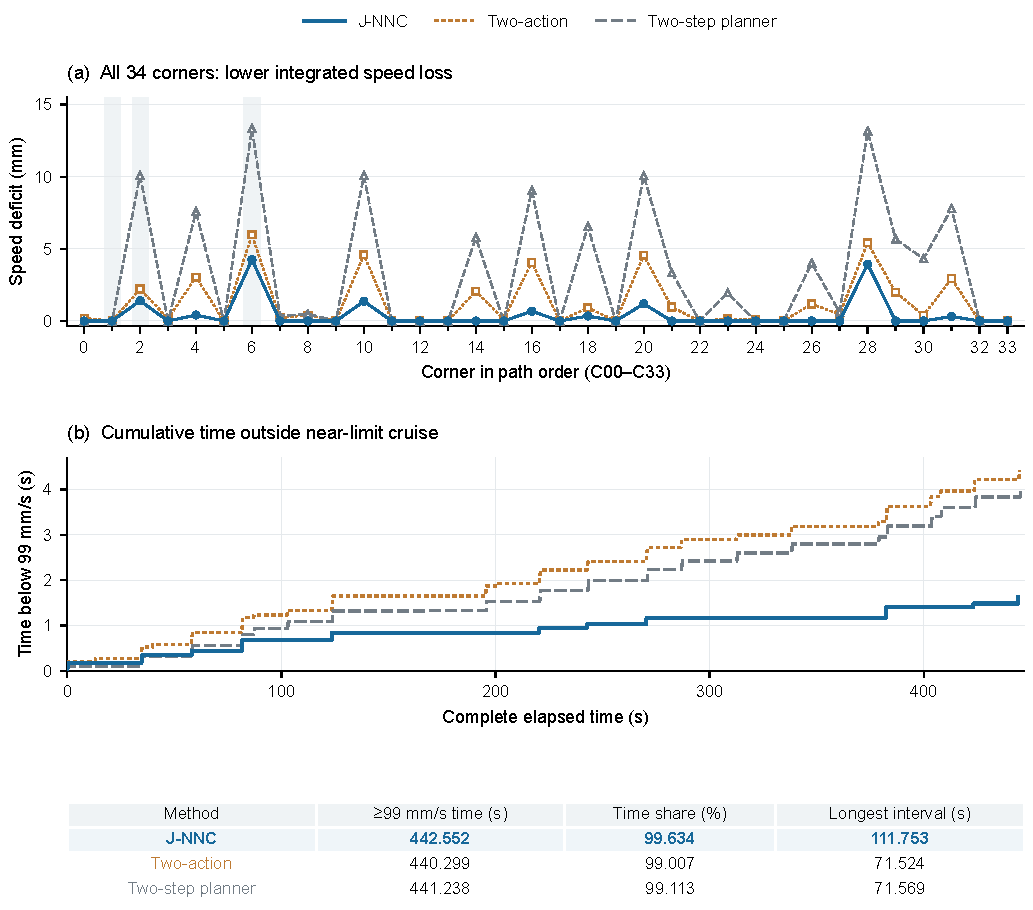
\includegraphics[width=0.98\linewidth]{Figure_8.pdf}
\caption{Corner speed deficits and full-path cruising at 1 ms: (a) integrated speed deficit in each $\pm10$ mm corner window, with representative corners shaded; (b) cumulative time below 99 mm/s. The inset table gives time at or above 99 mm/s, its fraction of complete execution time and the longest continuous interval. All 34 corners and terminal rest are included.}
\label{fig:all_corners}
\end{figure}

J-NNC spent 442.552 s at or above 99 mm/s, compared with 441.238 s for two-step planning and 440.299 s for two-action control. The longest continuous cruising intervals were 111.753, 71.569 and 71.524 s, respectively. Lower corner speed deficit coincided with longer sustained cruising and shorter complete execution time.

To distinguish path shortening from speed effects, let $L_{\mathrm{exec}}=h\sum_k\|v_k\|_2$ be executed path length and $D_{\mathrm{all}}=h\sum_k(100-\|v_k\|_2)$ be the full-path integrated speed deficit. Both sums cover all execution steps, including rest. Complete execution time $T$ then satisfies, up to floating-point roundoff,
\begin{equation}
T=\frac{L_{\mathrm{exec}}+D_{\mathrm{all}}}{100}.
\label{eq:time_decomposition}
\end{equation}
The terminal rest period is included in $D_{\mathrm{all}}$. J-NNC traveled 44390.406 mm with a total speed deficit of 27.294 mm; the two-step planner traveled 44392.151 mm with a deficit of 126.349 mm. Of the 1.008 s saved, approximately 0.991 s came from lower speed deficit and 0.017 s from shorter travel. Against the two-action controller, the 0.537 s saving comprised 0.303 s from lower speed deficit and 0.234 s from shorter travel. The dense case examines performance when successive transitions occupy a larger fraction of the path.

\subsection{Comparison with Fixed-Preview Control}
J-NNC completed the dense path in 14.839 s, compared with 15.875 s for the selected two-action controller. This corresponds to a 6.53\% reduction under the same physical constraints. Against the fastest valid two-action result among all evaluated models, 15.798 s, J-NNC saved 0.959 s (6.07\%).

\begin{figure}[!htbp]
\centering
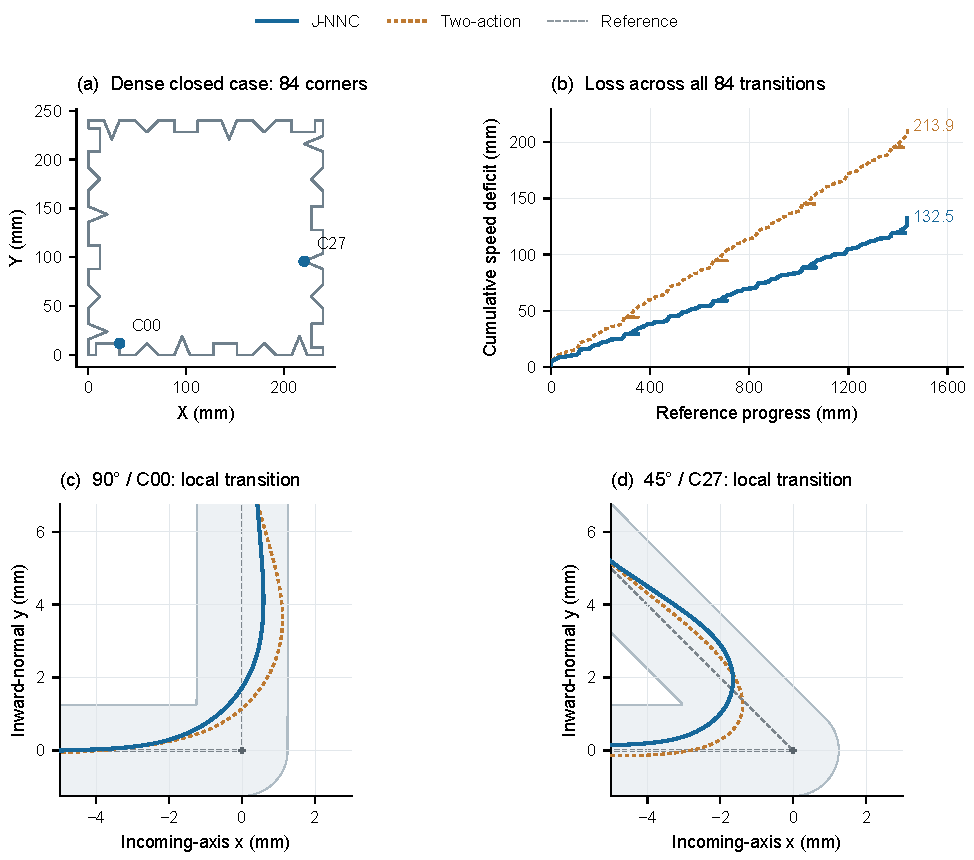
\includegraphics[width=0.98\linewidth]{Figure_9.pdf}
\caption{Comparison with two-action control at 1 ms: (a) dense closed path and locations of the local comparisons; (b) cumulative speed deficit over the complete execution, including all 84 corners and stopping; (c,d) executed $90^\circ$ and $45^\circ$ transitions. The curves correspond to the controllers in \tabref{tab:main_results}.}
\label{fig:ablation_dense}
\end{figure}

The local views in \figref{fig:ablation_dense}(c,d) show how the controllers use the tolerance band. J-NNC achieved 4.368 s of near-limit cruising on the dense path, compared with 0.114 s for the selected two-action controller. Total speed deficit decreased from 213.867 to 132.502 mm. Of the 1.036 s saved, 0.814 s came from lower speed deficit and 0.222 s from shorter travel. Both shorter travel and lower speed deficit contributed to the time saving. An equal-budget PPO comparison is reported in \ref{app:learning}.

Table~\ref{tab:selected_models} reports execution times by model ID. All listed models satisfied the motion constraints, completed both paths and met the speed-deficit criterion at all 34 long-path corners, with dense-case gains of 5.94\%--6.07\%. All main figures use model 923202.

\begin{table}[htbp]
\centering
\caption{Complete execution times by model ID at 1 ms. All satisfy the physical constraints, completion requirements and all-corner criteria. Dense-case gains are relative to the fastest valid two-action time of 15.798 s.}
\label{tab:selected_models}
\small
\begin{tabular}{lrrr}
\toprule
Model ID & Long path (s) & Dense case (s) & Dense gain (\%)\\
\midrule
923201 & 444.178 & 14.859 & 5.94\\
923202 (main) & 444.177 & 14.839 & 6.07\\
923203 & 444.178 & 14.839 & 6.07\\
\bottomrule
\end{tabular}
\end{table}

The long-path results show sustained cruising and no increase in corner speed deficit relative to either baseline. The dense path, where consecutive corner transitions occupy a larger share of the route, showed a larger time saving.

\section{Conclusion}
\label{sec:conclusion}
This paper presented J-NNC for CNC motion planning along mixed CAM-generated paths under contour and kinematic constraints. The policy jointly selects steering, feedrate and Adaptive Preview to coordinate trajectory shaping and feedrate regulation. The planar KCM projects the combined request into motion satisfying the velocity, acceleration and jerk limits. The policy uses 14 current geometric and kinematic inputs without stored history.

The same selected model completed the 44.420514 m long path and the 84-corner dense path, including ordered traversal, braking and rest. Speed deficit at all 34 long-path corners was no greater than for two-step planning or trained two-action control; complete execution time was 444.177 s. Dense-path execution took 14.839 s, reducing time by 6.07\% relative to the fastest valid two-action result and by 25.65\% relative to two-step planning. The local trajectories and V/A/J profiles show turning before the corner, feedrate recovery and sustained near-limit cruising within the tolerance band.

Future work will examine servo lag, axis-level constraints and machining performance.

\appendix
\section{Kinematic Constraint Module}
\label{app:kcm}
J-NNC and the two-action controller use the same KCM. At interpolation step $k$, the module selects a feasible next velocity $w$ from the execution layer's velocity request. Given the current velocity $v_k$, acceleration $a_k$ and interval $h$, the V/A/J constraints define the feasible set
\begin{equation}
\mathcal C_k=B(0,100)\cap B(v_k,1998h)\cap B(v_k+h a_k,62437.5h^2),
\label{eq:disks}
\end{equation}
where $B(c,r)$ is a closed disk with center $c$ and radius $r$. The three disks constrain speed, velocity change and acceleration change, respectively. Internal acceleration and jerk limits leave margins below 2000 mm/s$^2$ and 62500 mm/s$^3$. Candidate enumeration projects the velocity request onto their intersection.

A release check also requires a feasible subsequent reduction of acceleration along a straight line or constant-speed turn. For successive velocity vectors of magnitude $r>0$, let $d$ and $d'$ be consecutive angular increments. If their signs agree and $|d'|\leq|d|$, next-step jerk $j_{\mathrm{next}}$ satisfies
\begin{equation}
\|j_{\mathrm{next}}\|_2\leq \frac{\|a\|_2^2}{r}+\frac{r|d'-d|}{h^2}.
\end{equation}
For the release-check jerk bound $B=62375$ mm/s$^3$ and $\|a\|_2^2/r<B$, the angular increment is reduced by
\begin{equation}
|d|-|d'|=\min\!\left\{|d|,\frac{h^2}{2r}\left(B-\frac{\|a\|_2^2}{r}\right)\right\}.
\end{equation}
Each candidate is checked against the internal constraints. When speed already equals the requested 100 mm/s, projection includes feasible points on the constant-speed circle and selects the point closest to the velocity request. Otherwise, disk projection and a verified fallback determine the next state.

Algorithm~\ref{alg:kcm} summarizes the execution procedure.

\begin{algorithm}[H]
\caption{Complete execution with KCM constraints}
\label{alg:kcm}
\begin{algorithmic}[1]
\Require Ordered reference and current $(x_k,v_k,a_k)$
\While{reference coverage is incomplete and no failure has occurred}
\State At each decision update, encode the 14 current inputs and evaluate the policy
\State Decode $(\alpha,F,L)$ and hold for 20 ms
\For{each integration step before the next decision or termination}
\State Update guide direction and filtered desired velocity
\State Form the bounded jerk and next-velocity requests
\State Construct the three disks in Eq.~\eqref{eq:disks}
\State Project the request and check straight-line or constant-speed acceleration release
\State If necessary, search from a verified feasible fallback state
\State Set $a_{k+1}=(v_{k+1}-v_k)/h$ and $x_{k+1}=x_k+h v_{k+1}$
\State Update ordered coverage and check geometric feasibility
\EndFor
\EndWhile
\If{reference coverage is complete and no failure has occurred}
\State Execute nonreversing braking and at least 20 ms rest
\EndIf
\State Check geometry throughout each command interval and reconstruct vector motion from planar positions
\end{algorithmic}
\end{algorithm}

\section{Policy Representation and Learning Settings}
\label{app:learning}
\setcounter{table}{0}
\subsection{Policy Representation}
The base actor $m_\theta(s)$ has layers $14$--$64$--$64$--$3$ with hyperbolic tangent ($\tanh$) hidden activations; the critic has layers $14$--$64$--$64$--$1$. The preview and joint-action terms use static feature vectors $\phi^L(s)$ and $\phi^J(s)$ with 96 and 192 components, respectively. Centers $c_i$, positive coordinate scales $\sigma$ and support radii $r_i$ define
\begin{equation}
d_i=\|(s-c_i)/\sigma\|_2/r_i,\qquad
\phi_i(s)=\max(1-d_i,0)^4(4d_i+1).
\end{equation}
With preview coefficient row $w_L$, joint coefficient matrix $W$, and $e_3=(0,0,1)^{\mathsf T}$, deterministic execution uses
\begin{equation}
\begin{split}
\mu_\theta(s)&=m_\theta(s)+0.4e_3\tanh(w_L\phi^L(s))\\
&\quad+\operatorname{diag}(0.01,0.08,0.4)\tanh(W\phi^J(s)),\\
u&=\operatorname{clip}_{[-c,c]}(\mu_\theta(s)),\qquad c=1-10^{-10}.
\end{split}
\end{equation}
Clipping precedes decoding in Eq.~\eqref{eq:decode}, with a small margin to avoid numerical endpoints. The actor contains 5987 fitted network and output coefficients. Both feature banks use only the current 14 inputs, with one shared radius per bank. PPO samples a diagonal Gaussian centered on $\mu_\theta$; execution uses its mean.

\subsection{Learning Procedure}
Learning combines PPO with fitting to feasible actions recorded from an earlier policy. Action fitting alternates with four PPO stages of 16, 24, 24 and 24 updates. The final stage uses Eq.~\eqref{eq:reward_total} and batches of 1536 long-path and 512 dense-path decisions; earlier stages also include speed deficit.

The critic fits undiscounted returns and bootstraps from its value estimate at the end of unfinished segments. Each actor update combines the clipped PPO loss with a recorded-action fitting loss (\tabref{tab:ppo_details}), recomputes advantages and applies Kullback--Leibler (KL) backtracking.

\begin{table}[htbp]
\centering
\caption{Parameters of the last PPO training stage.}
\label{tab:ppo_details}
\small
\begin{tabular}{p{0.52\linewidth}p{0.38\linewidth}}
\toprule
Setting & Value\\
\midrule
Actor proposal learning rate / critic rate & $3\times10^{-4}$ / $10^{-3}$\\
PPO ratio clip / entropy coefficient & 0.2 / 0.001\\
Discount / advantage parameter & 1 / 0.98\\
Actor epochs / critic epochs & 6 / 32\\
Minibatch / fresh batch decisions & 256 / 2048\\
Actor / critic gradient norm limits & 0.5 / 1.0\\
Post-update divergence limit & 0.03\\
Auxiliary action-fit weight & 0.5\\
Auxiliary coordinate scales & $(0.015,0.15,0.3)$\\
\bottomrule
\end{tabular}
\end{table}

Final fitting holds feature centers and radii fixed and uses 12000 adaptive moment estimation (Adam) iterations. The learning rate starts at $2\times10^{-4}$ and is multiplied by 0.3 at iterations 4000 and 8000. Each batch contains 256 records per case; loss scales are $(0.015,0.15,0.3)$ and the gradient limit is 1.

\subsection{Comparison Settings}
The two-action actor has layers $14$--$64$--$64$--$2$, 192 joint features and 5634 coefficients. It uses the first two correction scales and identical clipping. Fixed preview $L=3$ mm was selected from $\{1.5,3,4.5,6,8,12\}$ mm before fitting and PPO training. The controllers use different training schedules and budgets.

The models in Table~\ref{tab:selected_models} share recorded-action data and use the same static-feature formulation, with model-specific refinement settings.

A separate matched PPO comparison starts with identical steering/feedrate requests and constant preview. Each controller receives 48 updates and 98304 new decisions; updates 0, 24 and 48 are evaluated on both paths and interpolation intervals. Successful checkpoints are ranked by worst normalized time, then mean normalized time and update index; the initial model is retained if no improvement occurs. Action standard deviations are $(0.002,0.015,0.02)$ and the action-fit weight is 0.25. Execution-time differences remain within the numerical sensitivity margin.

\begin{figure}[H]
\centering
\renewcommand{\thefigure}{B.\arabic{figure}}
\setcounter{figure}{0}
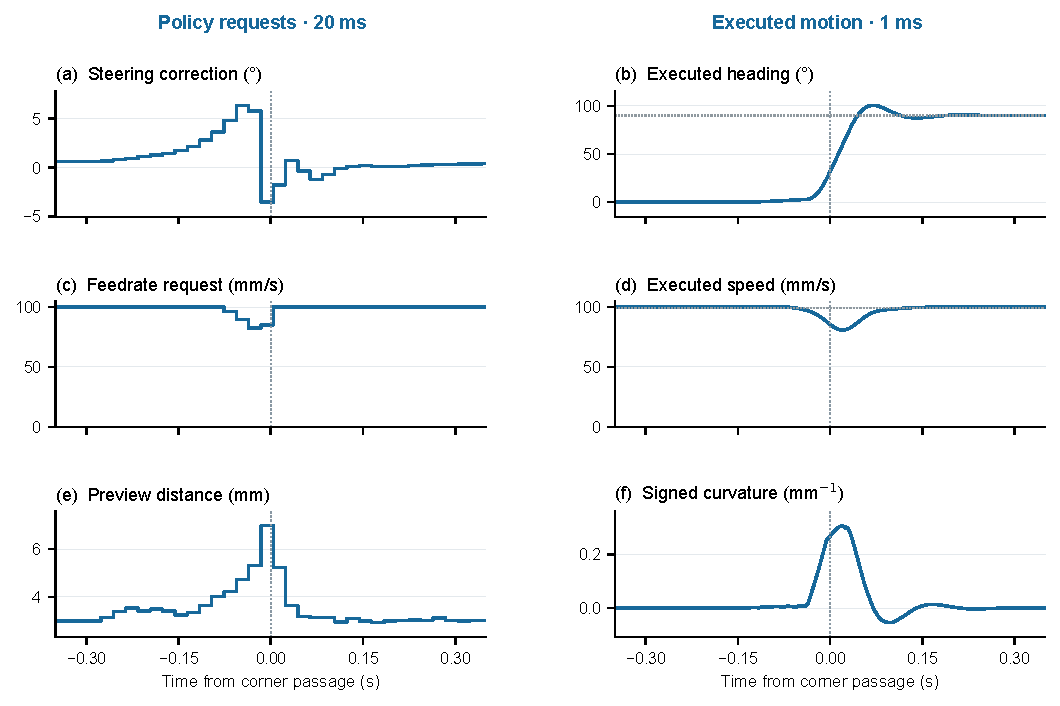
\includegraphics[width=0.96\linewidth]{Figure_B1.pdf}
\caption{Actions and executed motion at the $90^\circ$/C02 corner in Fig.~\ref{fig:full_utilization}. Left: steering correction, feedrate request and preview distance held between 20 ms updates. Right: heading, speed and signed curvature from 1 ms positions. Time $t=0$ marks the first sample reaching the corner in ordered progress. Heading is relative to the incoming tangent; steering, heading and curvature are positive inward. Dotted lines mark the outgoing $90^\circ$ heading and 99 mm/s cruising threshold. Signals are unsmoothed and share the time axis.}
\label{fig:action_correspondence}
\end{figure}

\setlength{\bibsep}{3pt plus 0.3pt}

\section{Execution-Resolution Check}
\label{app:resolution}
\setcounter{table}{0}
Evaluations were repeated at $h=0.5$ ms with unchanged policy parameters, physical limits and 20 ms decisions (Table~\ref{tab:resolution}). All listed constrained controllers remained feasible. Maximum J-NNC contour deviation was 1.249077 mm on the dense path, within the 1.25 mm tolerance.

\begin{table}[htbp]
\centering
\caption{Complete execution times at 0.5 ms. The primary comparison at 1 ms is given in \tabref{tab:main_results}.}
\label{tab:resolution}
\small
\begin{tabular}{lrrr}
\toprule
Case & J-NNC (s) & Two-action (s) & Two-step planner (s)\\
\midrule
Long path & 444.1950 & 444.7310 & 445.1850\\
Dense case & 14.8785 & 15.8955 & 19.9565\\
\bottomrule
\end{tabular}
\end{table}

Let $\delta T$ be the absolute execution-time change between 1 and 0.5 ms. The numerical sensitivity criterion requires gains at both intervals to exceed $\max\{0.100,5(\delta T_{\mathrm{J\text{-}NNC}}+\delta T_{\mathrm{baseline}})\}$ seconds, where the subscripts identify the compared controllers. Long-path gains were 1.008/0.990 s over two-step planning and 0.537/0.536 s over two-action control, exceeding margins of 0.100 and 0.175 s. Dense-path gains over the fastest valid two-action times (15.798/15.8755 s) were 0.959/0.997 s, exceeding the 0.585 s margin.

The result for all 34 corners held at both intervals with wider $\pm20$ and $\pm30$ mm windows. At 0.5 ms, models 923201, 923202 and 923203 completed the long path in 444.1955, 444.1950 and 444.1955 s, and the dense path in 14.8980, 14.8785 and 14.8775 s. All met feasibility and corner criteria; dense-path gains over the fastest valid two-action result were 6.16\%--6.29\%.

\begin{figure}[H]
\centering
\renewcommand{\thefigure}{C.\arabic{figure}}
\setcounter{figure}{0}
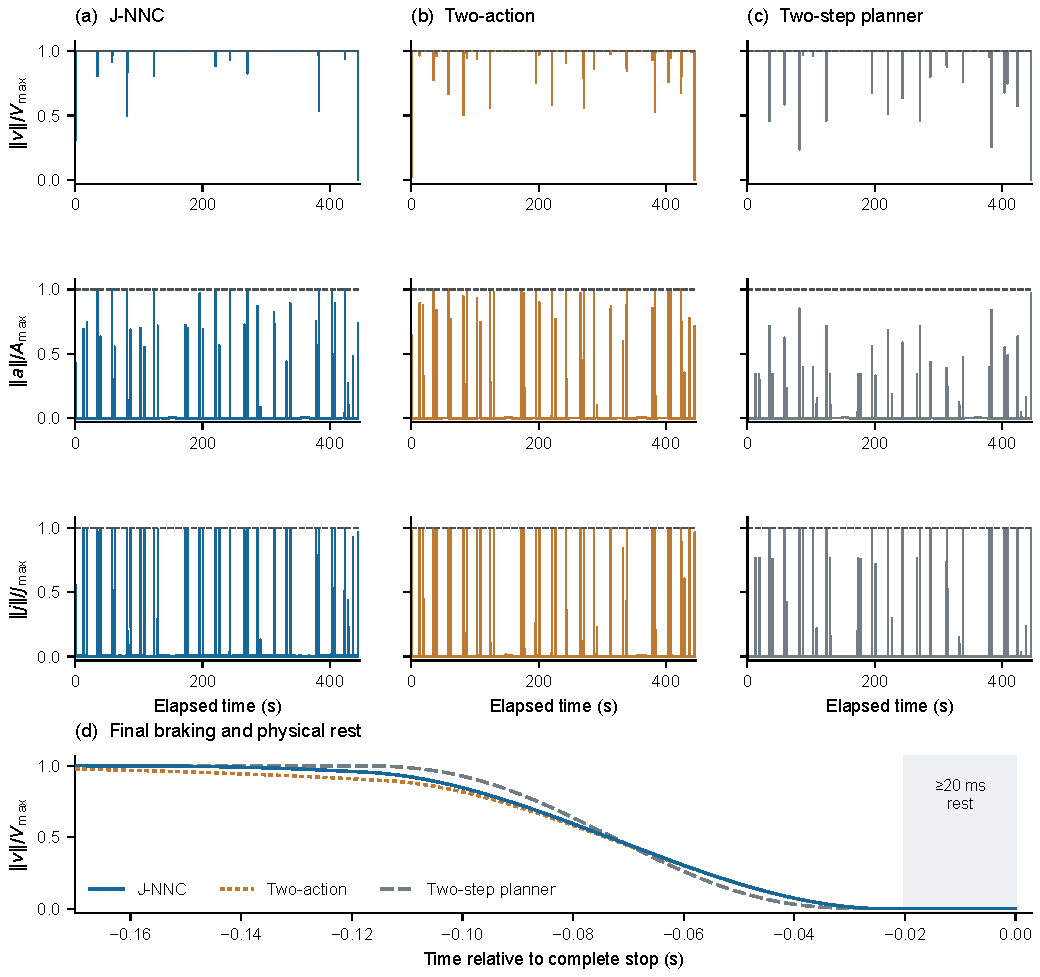
\includegraphics[width=0.98\linewidth,height=0.75\textheight,keepaspectratio]{Figure_C1.pdf}
\caption{Complete long-path profiles at 1 ms. Columns: J-NNC, two-action control and two-step planning. Rows: normalized vector speed, acceleration and jerk. Plot downsampling preserves minima and maxima; the lower panel includes braking and at least 20 ms of rest.}
\label{fig:complete_support}
\end{figure}

\bibliographystyle{apacite}
\bibliography{references}
\end{document}
